\section{Layout}

\begin{figure}[H]
    \hspace*{-2cm}
    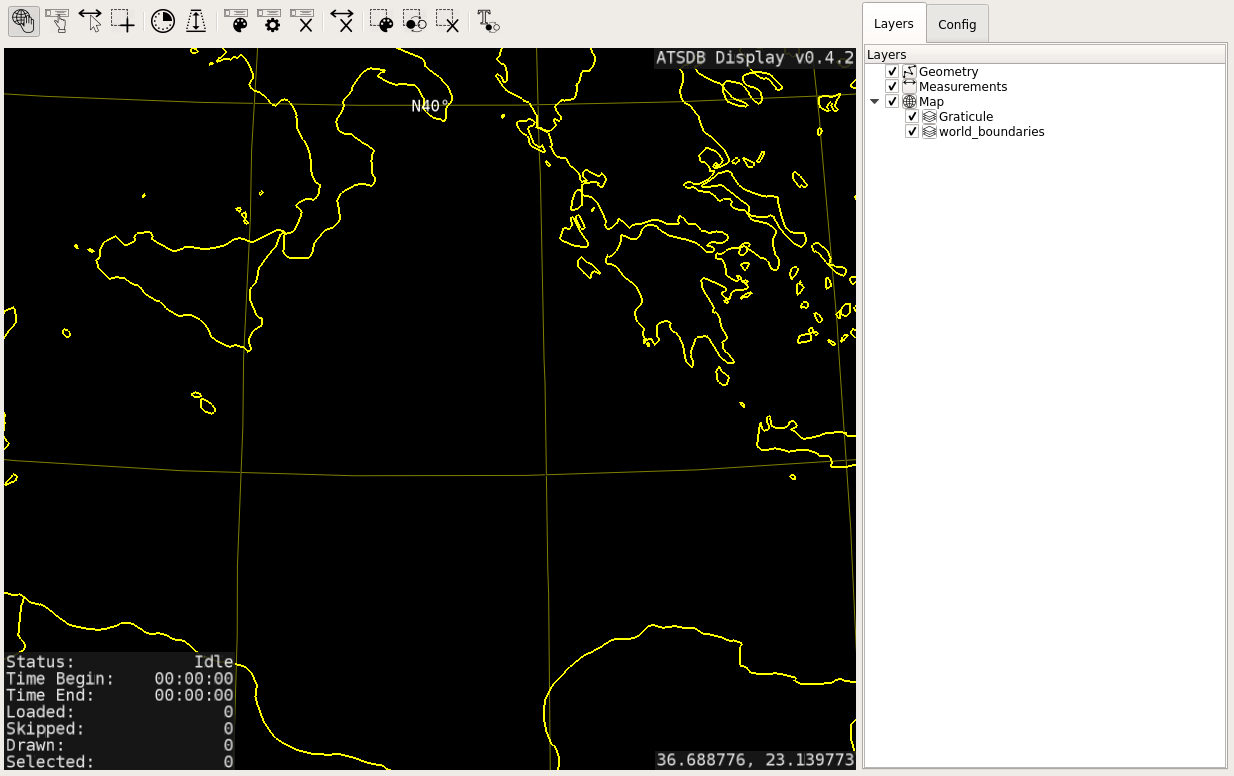
\includegraphics[width=18cm,frame]{../screenshots/osgview_overview.png}
  \caption{OSG View overview}
  \label{fig:osgview_overview}
\end{figure}

The map window will automatically traverse to the medium location of the data in the current database. \\

There exist 3 main components:
\begin{itemize}
 \item Toolbar (top left): Selects mouse action or set display options.
 \item Data Widget (lower left): Displays map and geometry data.
 \item Configuration panel (right): Displays layer and configuration tabs.
\end{itemize}
\ \\

To load the data use the the mechanism described in Section \nameref{sec:management_dbos} can be used. To filter the dataset, the mechanism described in Section \nameref{sec:filtering} can be used. \\

After loading, the target reports will be shown.

\begin{figure}[H]
    \hspace*{-2cm}
    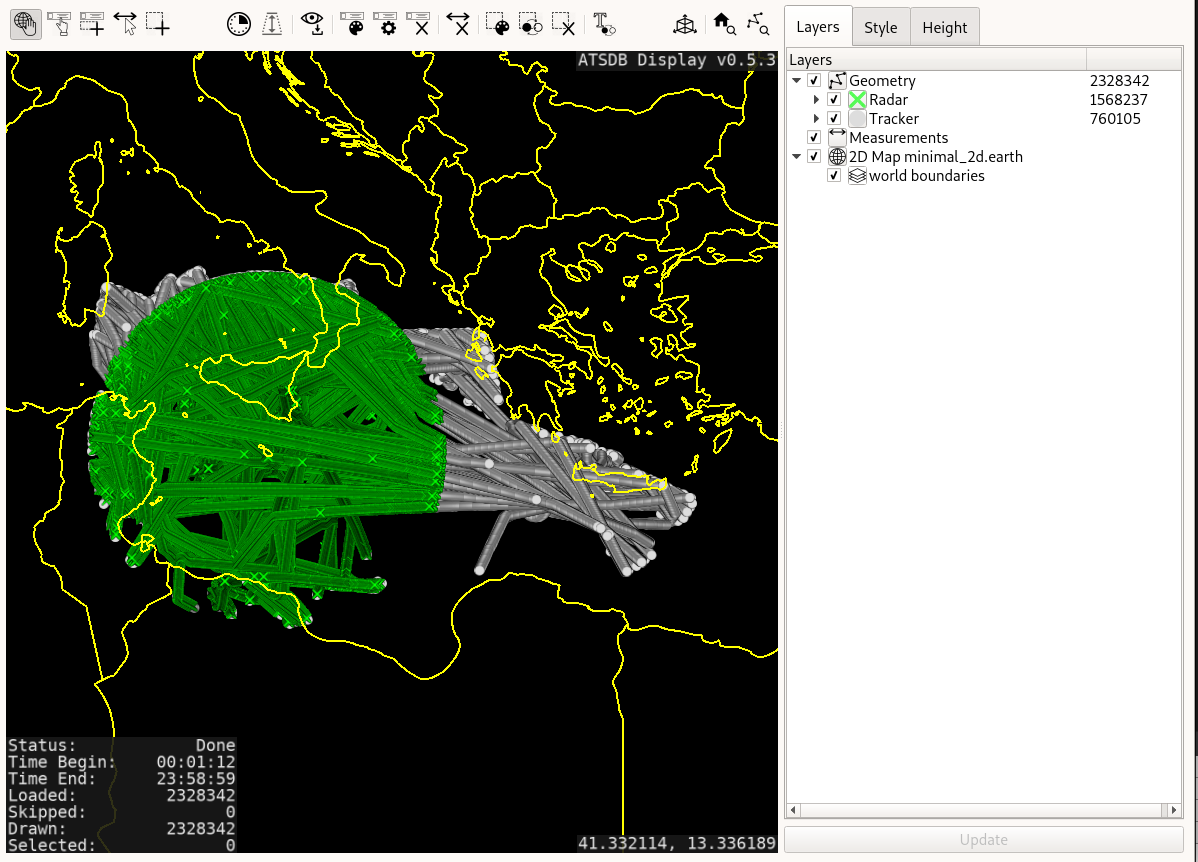
\includegraphics[width=18cm,frame]{../screenshots/osgview_overview_loaded.png}
  \caption{OSG View overview after loading}
\end{figure} 

How the data is presented in defined in the Configuration tab, please refer to \nameref{sec:osgview_config} for details. \\

For each DBO, a default display configuration is set:

\begin{itemize}
 \item Tracker: White circle (default)
 \item Radar: Green cross (default)
 \item MLAT: Red triangle (default)
 \item ADS-B: Blue square (default)
\end{itemize}
